% Created 2013-03-02 Sat 17:25
\documentclass[presentation]{beamer}
\usepackage[utf8]{inputenc}
\usepackage[T1]{fontenc}
\usepackage{fixltx2e}
\usepackage{graphicx}
\usepackage{longtable}
\usepackage{float}
\usepackage{wrapfig}
\usepackage{soul}
\usepackage{textcomp}
\usepackage{marvosym}
\usepackage{wasysym}
\usepackage{latexsym}
\usepackage{amssymb}
\usepackage{hyperref}
\tolerance=1000
\institute{The Really Great Institute \\ Somewhere On, Earth}
\usetheme{default}
\usecolortheme{beaver}
\author{G. Jay Kerns}
\date{\today}
\title{Sample \texttt{julia} Presentation}
\hypersetup{
  pdfkeywords={},
  pdfsubject={},
  pdfcreator={Generated by Org mode 7.9.3f in Emacs 24.3.50.1.}}
\begin{document}

\maketitle
\begin{frame}{Outline}
\tableofcontents
\end{frame}


\section[A Sample \texttt{julia} Beamer presentation]{A Sample \texttt{julia} Beamer presentation}
\label{sec-1}

\begin{frame}[fragile,label=sec-1-1]{}
 For this to successfully export to PDF you'll need

\begin{verbatim}
(require 'ox-beamer)
\end{verbatim}

and you'll need a Beamer entry similar to this

\begin{verbatim}
(add-to-list 'org-latex-classes
	     '("beamer"
        "\\documentclass[presentation]{beamer}
        \[DEFAULT-PACKAGES]
        \[PACKAGES]
        \[EXTRA]"
	       ("\\section{%s}" . "\\section*{%s}")
	       ("\\subsection{%s}" . "\\subsection*{%s}")
	       ("\\subsubsection{%s}" . "\\subsubsection*{%s}")))
\end{verbatim}

in your \texttt{.emacs}. Then open the org file and do: \texttt{C-c C-e l P}.
\end{frame}
\begin{frame}[fragile,label=sec-1-2]{Frame 1}
 \framesubtitle{Two blocks with a pause in between, noweb reference}
\begin{columns}
\begin{column}{0.5\textwidth}
\begin{block}{Here is some \texttt{julia} code}

\label{simple-code}
\begin{verbatim}
2+3
print("hello, there!")
sqrt(5)
\end{verbatim}

\pause
\end{block}
\end{column}
\begin{column}{0.5\textwidth}
\begin{block}{Here is the output}

\begin{verbatim}
5
hello, there!
2.23606797749979
\end{verbatim}
\end{block}
\end{column}
\end{columns}
\note{This is a beamer note
This subtree will not appear in the PDF. Notice the noweb call \texttt{<<simple-code>>} which is replaced by the named \texttt{simple-code} src block above (so we don't have to type the same code twice).  It is activated by the \texttt{:noweb yes} header argument. You will notice those headline tags, such as \texttt{:BMCOl:B\_block:} and \texttt{:B\_note:}.  Don't fret about those; they are just a visual aid.}
\end{frame}
\begin{frame}[fragile,label=sec-1-3]{Frame 2}
 \framesubtitle{Horizontal block, text (list) animations, footnotes, hyperlinks}

\begin{block}{This block extends horizontally}
Be sure to put 

\begin{verbatim}
#+PROPERTY: session *julia*
\end{verbatim}

at the top of the org file to ensure \texttt{julia} code block session evalation by default.
\end{block}
\begin{itemize}[<+->]
\item Enter Column View\footnote{See \href{http://thread.gmane.org/gmane.emacs.orgmode/5107/focus=5134}{this message} on Gmane for more about Column View.} with \texttt{C-c C-x C-c} on headline
\item Might like \texttt{S-TAB} to collapse headlines first
\item Handy for editing headline properties
\item Set \texttt{ignoreheading} with \texttt{C-c C-b i} on headline
\end{itemize}
\end{frame}
\begin{frame}[fragile,label=sec-1-4]{Frame 3}
 \framesubtitle{Images and captions, font tweaks for source code}

\begin{columns}
\begin{column}{0.6\textwidth}
\begin{block}{The \texttt{julia} code}

\footnotesize

\begin{verbatim}
using Winston
x = linspace(0, 3pi, 100)
c = cos(x)
s = sin(x)
p = FramedPlot();
setattr(p, "title", "title!")
setattr(p, "xlabel", L"\Sigma x^2_i")
setattr(p, "ylabel", L"\Theta_i")
add(p, FillBetween(x, c, x, s) )
add(p, Curve(x, c, "color", "red") )
add(p, Curve(x, s, "color", "blue") )
file(p, "example1.pdf")
\end{verbatim}

\normalsize
\end{block}
\end{column}
\begin{column}{0.4\textwidth}
\begin{block}{The image}

\begin{figure}[htb]
\centering
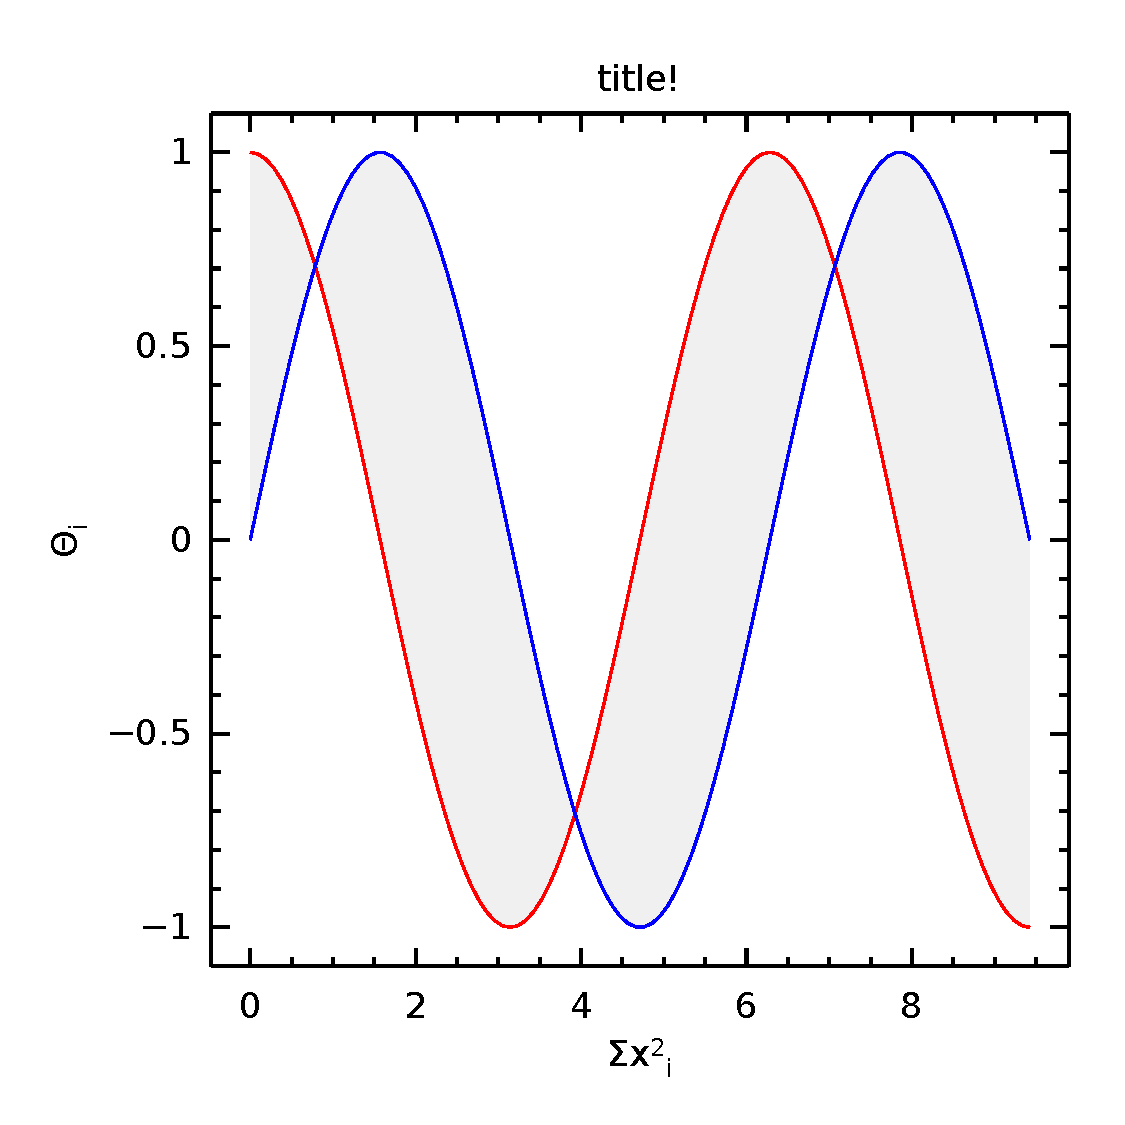
\includegraphics[width=.9\linewidth]{example1.pdf}
\caption{A \texttt{julia} graph}
\end{figure}
\end{block}
\end{column}
\end{columns}
\end{frame}
\begin{frame}[allowframebreaks,label=sec-1-5]{References}
\framesubtitle{Write this one in pure LaTeX and \texttt{allowframebreaks}}

\begin{thebibliography}{10}    
\beamertemplatearticlebibitems
\bibitem{Guy2013}
  R. Smart Guy.
  \newblock This theorem is hard to prove.
  \newblock {\em Journal of Difficult Things}, 5(7):91--97, 2013.
\beamertemplatebookbibitems
\bibitem{Important2012}
  Somebody R. Important.
  \newblock {\em A Heavy Book}.
  \newblock Bigtime-Publisher, 2012.
\beamertemplatearrowbibitems
\bibitem{beamerexport}
  Beamer Class Export.
  \newblock The Org Manual.
  \newblock \url{http://orgmode.org/manual/Beamer-class-export.html}
\bibitem{beameroldengine}
  Writing Beamer presentations in org-mode.
  \newblock The link is on Worg \href{http://orgmode.org/worg/exporters/beamer/tutorial.html}{\emph{here}}. Also see \href{http://orgmode.org/worg/exporters/beamer/ox-beamer.html}{\emph{here}} for info regarding the new exporter.
\end{thebibliography}
\end{frame}
% Generated by Org mode 7.9.3f in Emacs 24.3.50.1.
\end{document}